
杀毒器是一种检查编译器插入的代码(检测)的某些运行时技术。人们通常使用杀毒器来确保程序的正确性或执行安全策略。为了了解消毒剂是如何工作的,让我们以Clang中最流行的杀毒器为例——\textbf{地址杀毒器(address sanitizer)}。

\subsubsubsection{12.2.1\hspace{0.2cm}使用地址杀毒器的例子}

假设我们有一些简单的C代码,例如:

\begin{lstlisting}[style=styleCXX]
int main(int argc, char **argv) {
	int buffer[3];
	for (int i = 1; i < argc; ++i)
		buffer[i-1] = atoi(argv[i]);
		
	for (int i = 1; i < argc; ++i)
		printf("%d ", buffer[i-1]);
	printf("\n");
	return 0;
}
\end{lstlisting}

前面的代码将命令行参数转换为整数,并将它们存储在大小为3的缓冲区中。然后,把它们打印出来。

应该能够很容易地发现一个突出的问题:当\texttt{argc}的值大于3(缓冲区的大小)时,它的值可以任意大。这里,会将值存储在一个无效的内存位置。然而,编译这段代码时,编译器什么都不会报告。下面是一个例子:

\begin{tcblisting}{commandshell={}}
$ clang -Wall buffer_overflow.c -o buffer_overflow
$ # No error or warning
\end{tcblisting}

命令中,即使我们通过\texttt{-Wall}标志启用了所有的编译器警告,\texttt{clang}也不会抱怨存在的错误。

如果尝试执行\texttt{buffer\_overflow}时,当我们向它传递三个以上的命令行参数后,程序将会崩溃:

\begin{tcblisting}{commandshell={}}
$ ./buffer_overflow 1 2 3
1 2 3
$ ./buffer_overflow 1 2 3 4
Segmentation fault (core dumped)
$
\end{tcblisting}

更糟糕的是,崩溃\texttt{buffer\_overflow}的命令行参数的数量实际上因机器而异,那么调试就会更加困难。总之,我们在这里遇到的问题是:\texttt{buffer\_overflow}只会在某些输入上出错,而编译器未能捕捉到这个问题。 

现在,让我们试着用一个地址杀毒器来捕捉这个bug。下面的命令要求\texttt{clang}用地址杀毒器编译相同的代码:

\begin{tcblisting}{commandshell={}}
$ clang -fsanitize=address buffer_overflow.c -o san_buffer_overflow
\end{tcblisting}

让我们再次执行这个程序。输出如下:

\begin{tcblisting}{commandshell={}}
$ ./san_buffer_overflow 1 2 3
1 2 3
$ ./san_buffer_overflow 1 2 3 4
==============================================================
===
==137791==ERROR: AddressSanitizer: stack-buffer-overflow on
address 0x7ffea06bccac at pc 0x0000004f96df bp 0x7ffea06bcc70…
WRITE of size 4 at 0x7ffea06bccac thread T0
…
  This frame has 1 object(s):
    [32, 44) 'buffer' <== Memory access at offset 44 overflows this variable
…
==137791==ABORTING
$
\end{tcblisting}

除了崩溃,地址杀毒器还向我们提供了关于运行时提出的问题的许多细节:杀毒器告诉我们,检测到堆栈上的缓冲区溢出,这可能是缓冲区变量。

这些信息非常有用。假设正在处理一个复杂得多的软件项目时,当一个奇怪的内存错误发生时,而不是仅仅崩溃或改变程序的逻辑,地址杀毒器可以指出有问题的区域,且具有很高的准确性。

为了更深入地了解它的机制,下面的图表说明了地址杀毒器如何检测缓冲区溢出:

\hspace*{\fill} \\ %插入空行
\begin{center}
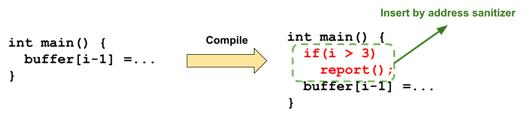
\includegraphics[width=0.7\textwidth]{content/3/chapter12/images/1.png}\\
图12.1 -地址杀毒器插入的检测代码
\end{center}

这里,可以看到地址杀毒器正在有效地将边界检查,插入到用于访问缓冲区的数组索引中。通过这个检查(将在运行时执行),目标程序可以在违反内存访问之前带着错误详细信息退出。更一般地说,在编译期间,杀毒器将插入一些检测代码(到目标程序中),这些代码最终将在运行时执行,以检查或保护某些属性。

\begin{tcolorbox}[colback=blue!5!white,colframe=blue!75!black, fonttitle=\bfseries,title=使用地址杀毒器检测溢出]	
\hspace*{0.7cm}上面的图表显示了地址杀毒器工作原理的简化版本。实际上,地址杀毒器会利用多种策略来监视程序中的内存访问,例如:地址杀毒器可以使用一个特殊的内存分配器来分配内存,并在无效的内存区域放置陷阱。
\end{tcolorbox}

虽然地址杀毒器专门用于捕获非法内存访问,但\textbf{ThreadSanitizer}可以用于捕获数据竞争条件,也就是多个线程对同一块数据的无效访问。Clang中的杀毒器的其他例子是\textbf{LeakSanitizer},用于检测敏感数据,如:密码泄露。以及\textbf{MemorySanitizer},用于检测对未初始化内存的读取。

当然,使用杀毒器也有一些缺点。最突出的问题是性能影响:以线程杀毒器(Clang内置的)为例,用一个线程杀毒器编译的程序比原始版本慢5~15倍。而且,由于杀毒器会向程序中插入额外的代码,这可能会阻碍一些优化机会,甚至会影响原始程序的逻辑!换句话说,这是在目标程序的健壮性和性能之间的权衡。

至此,我们了解了杀毒器的概念。现在,可以尝试自己创建一个杀毒器,以理解Clang和LLVM如何实现杀毒器器。下一节包含的代码比前几章的任何示例都要多,更不用说LLVM中不同子项目之间的变更了。为了关注最重要的知识点,我们不会深入一些支持代码的细节——例如,对CMake构建脚本所做的更改。相反,我们将提供一个简短的介绍,并指出在本书的GitHub库中,你可以在哪里找到它。

让我们从概述将要创建的项目开始。


\subsubsubsection{12.2.2\hspace{0.2cm}创建循环计数器杀毒器}

为了(稍微)简化我们的任务,将要创建的杀毒器(循环计数器杀毒器,简称\textbf{LPCSan})看起来就像杀毒器,只是它不检查任何重要的程序属性。相反,我们希望使用它来打印一个循环的真实的、具体的计数(迭代次数),这只能在运行时可用。

例如,我们有以下输入代码:

\begin{lstlisting}[style=styleCXX]
void foo(int S, int E, int ST, int *a) {
	for (int i = S; i < E; i += ST) {
		a[i] = a[i + 1];
	}
}
int main(int argc, char **argv) {
	int start = atoi(argv[1]),
	    end = atoi(argv[2]),
	    step = atoi(argv[3]);
	int a[100];
	foo(start, end, step, a);
	return 0;
}
\end{lstlisting}

我们可以使用LPCSan编译:

\begin{tcblisting}{commandshell={}}
$ clang -O1 -fsanitize=loop-counter test_lpcsan.c -o test_lpcsan
\end{tcblisting}

注意,编译时优化值大于\texttt{-O0}是必要的,稍后会解释原因。

当执行\texttt{test\_lpcsan}(带有一些命令行参数)时,我们可以在\texttt{foo}函数中打印出循环计数:

\begin{tcblisting}{commandshell={}}
$ ./test_lpcsan 0 100 1
==143813==INFO: Found a loop with trip count 100
$ ./test_lpcsan 0 50 2
==143814==INFO: Found a loop with trip count 25
$
\end{tcblisting}

以上代码的消息,是由我们的杀毒程序代码打印的。

现在,让我们深入了解创建LPCSan的步骤。我们将把这个过程分为三个部分:

\begin{itemize}
\item 开发IR转换
\item 添加Compiler-RT组件
\item 将LPCSan加入Clang
\end{itemize}

我们将从这个杀毒器的IR转换部分开始。


\hspace*{\fill} \\ %插入空行
\noindent
\textbf{开发IR转换}

前面,我们了解了地址杀毒器——或者只是一般的杀毒器——通常将代码插入到目标程序中,以检查特定的运行时属性或收集数据。在第9章和第10章中,我们了解了如何修改/转换LLVM IR,包括在其中插入新代码,所以这对于制作我们的LPCSan,是一个很好的入手点。

本节中,我们将开发一个名为\texttt{LoopCounterSanitizer}的LLVM Pass,它将插入特殊的函数调用来收集模块中每个循环的准确行程计数。具体步骤如下:

\begin{enumerate}
\item 首先,让我们创建两个文件:\texttt{llvm/lib/Transforms/Instrumentation}文件夹下的\texttt{LoopCoun terSanitizer.cpp}和\texttt{llvm/include/llvm/Transforms/Instrumentation}文件夹下的相应头文件。头文件中,我们将放置这个Pass的声明:

\begin{lstlisting}[style=styleCXX]
struct LoopCounterSanitizer
: public PassInfoMixin<LoopCounterSanitizer> {
	PreservedAnalyses run(Loop&, LoopAnalysisManager&,
						  LoopStandardAnalysisResults&,
						  LPMUpdater&);
private:
	// Sanitizer functions
	FunctionCallee LPCSetStartFn, LPCAtEndFn;
	void initializeSanitizerFuncs(Loop&);
};
\end{lstlisting}

上面的代码展示了我们在第10章中看到的典型循环传递结构。值得注意的变化是\texttt{LPCSetStartFn}和\texttt{LPCAtEndFn}内存变量——将存储收集循环次数的\texttt{Function}实例(\texttt{FunctionCallee}是一个包装函数,只提供额外的函数签名信息)。

\item 最后,在\texttt{LoopCounterSanitizer.cpp}中,我们实现了Pass的框架代码:

\begin{lstlisting}[style=styleCXX]
PreservedAnalyses
LoopCounterSanitizer::run(Loop &LP, LoopAnalysisManager
&LAM, LoopStandardAnalysisResults &LSR, LPMUpdater &U) {
	initializeSanitizerFuncs(LP);
	return PreservedAnalyses::all();
}
\end{lstlisting}

以上代码中的\texttt{initializeSanitizerFuncs}方法将赋予\texttt{LPCSetStartFn}和\texttt{LPCAtEndFn}。在我们深入\texttt{initializeSanitizerFunc}s的细节之前,让了解一下\texttt{LPCSetStartFn}和\texttt{LPCAtEndFn}。

\item 为了计算出准确的循环计数,将使用存储在\texttt{LPCSetStartFn}中的\texttt{Function}实例来收集循环的初始引导变量值。另一方面,存储在\texttt{LPCAtEndFn}中的\texttt{Function}实例,将用于收集最终的归纳变量值和循环的步长值。为了给有一个具体的概念,了解这两个函数实例是如何一起工作的,我们假设有以下伪代码作为输入程序:

\begin{lstlisting}[style=styleCXX]
void foo(int S, int E, int ST) {
	for (int i = S; i < E; i += ST) {
		…
	}
}
\end{lstlisting}

前面的代码中,\texttt{S}、\texttt{E}和\texttt{ST}变量分别表示循环的初始值、最终值和步长值。\texttt{LoopCounterSanitizer} Pass的目标是插入\texttt{LPCSetStartFn}和\texttt{LPCAtEndFn},方法如下:

\begin{lstlisting}[style=styleCXX]
void foo(int S, int E, int ST) {
	for (int i = S; i < E; i += ST) {
		lpc_set_start(S);
		…
		lpc_at_end(E, ST);
	}
}
\end{lstlisting}

以上代码中的\texttt{lpc\_set\_start}和\texttt{lpc\_at\_end}分别是存储在\texttt{LPCSetStartFn}和\texttt{lpccatendfn}的函数实例中。下面是这两个函数可能的(伪)实现:

\begin{lstlisting}[style=styleCXX]
static int CurrentStartVal = 0;
void lpc_set_start(int start) {
	CurrentStartVal = start;
}
void lpc_at_end(int end, int step) {
	int trip_count = (end – CurrentStartVal) / step;
	printf("Found a loop with trip count %d\n",
	trip_count);
}
\end{lstlisting}

现在我们已经了解了\texttt{LPCSetStartFn}和\texttt{LPCAtEndFn}的角色,接下来看看\texttt{initializeSan itizerFuncs}是如何初始化它们的。

\item 下面是\texttt{initializeSanitizerFuncs}内部代码:

\begin{lstlisting}[style=styleCXX]
void LoopCounterSanitizer::initializeSanitizerFuncs(Loop
&LP) {
	Module &M = *LP.getHeader()->getModule();
	auto &Ctx = M.getContext();
	Type *VoidTy = Type::getVoidTy(Ctx),
	     *ArgTy = Type::getInt32Ty(Ctx);
	LPCSetStartFn
	  = M.getOrInsertFunction("__lpcsan_set_loop_start",
	                          VoidTy, ArgTy);
	LPCAtEndFn = M.getOrInsertFunction("__lpcsan_at_loop_
	  end", VoidTy, ArgTy, ArgTy);
}
\end{lstlisting}

前面的代码基本上是从模块中获取两个函数,\texttt{\_\_lpcsan\_set\_loop\_ start}和\texttt{\_\_lpcsan\_at\_l oop\_end},并分别将它们的函数实例存储在\texttt{LPCSetStartFn}和\texttt{LPCAtEndFn}中。

\texttt{Module::getOrInsertFunction}要么从模块中获取给定函数名的\texttt{Function}实例,要么创建一个不存在的\texttt{Function}实例。如果是一个新创建的实例,它有一个空的函数体;换句话说,这就是一个函数声明。

同样值得注意的是,\texttt{Module::getOrInsertFunction}的第二个参数是\texttt{Function}查询的返回类型。其余的(\texttt{getOrInsertFunction}参数)表示该\texttt{Function}的参数类型。

设置了\texttt{LPCSetStartFn}和\texttt{LPCAtEndFn}后,我们来了解一下如何将它们插入到IR中的正确位置。

\item 在第10章中,我们了解了几个用于处理\texttt{Loop}的工具类。其中之一就是\texttt{LoopBounds},可以给出一个循环的边界。可以通过包含归纳变量的开始、结束和步长值来实现这一点,这正是我们要寻找的信息。下面是检索\texttt{LoopBounds}实例的代码:

\begin{lstlisting}[style=styleCXX]
PreservedAnalyses
LoopCounterSanitizer::run(Loop &LP, LoopAnalysisManager
&LAM, LoopStandardAnalysisResults &LSR, LPMUpdater &U) {
	initializeSanitizerFuncs(LP);
	ScalarEvolution &SE = LSR.SE;
	
	using LoopBounds = typename Loop::LoopBounds;
	auto MaybeLB = LP.getBounds(SE);
	if (!MaybeLB) {
		errs() << "WARNING: Failed to get loop bounds\n";
		return PreservedAnalyses::all();
	}
	LoopBounds &LB = *MaybeLB;
	…
	Value *StartVal = &LB.getInitialIVValue(),
		  *EndVal = &LB.getFinalIVValue(),
		  *StepVal = LB.getStepValue();
}
\end{lstlisting}

上面代码中的\texttt{Loop::getBounds}返回一个\texttt{Optional<LoopBounds>}实例。\texttt{Optional<T>}类是一个有用的容器,要么存储\texttt{T}类型的实例,要么为空。可以把它看作是空指针的替换:通常,用\texttt{T*}来表示计算结果,空指针时则为空值。但是,如果开发者忘记先检查空指针,就会有对空指针进行解引用的风险。\texttt{Optional<T>}类就没有这个问题。

使用\texttt{LoopBounds}实例,我们可以检索归纳变量的范围,并将其存储在\texttt{StartVal}、\texttt{EndVal}和\texttt{StepVal}变量中。

\item \texttt{StartVal}是由\texttt{\_\_lpcsan\_set\_loop\_ start}收集的\texttt{Value}实例,而\texttt{\_\_lpcsan\_at\_loop\_end}将在运行时收集\texttt{EndVal}和\texttt{StepVal}。现在,问题是,我们应该在哪里插入函数\texttt{\_\_lpcsan\_se t\_loop\_start}和\texttt{\_\_lpcsan\_at\_loop\_end}来正确地收集这些值呢?

根据经验,需要将这些函数调用插入到这些值的定义之后。虽然我们可以找到定义这些值的确切位置,但我们可以在一些固定的位置(目标值总是可用的位置)插入工具函数来尝试简化这个问题。

对于\texttt{\_\_lpcsan\_set\_loop\_start},我们将它插入到\textbf{循环头}块的末尾,因为初始的感应变量值永远不会在这个块之后定义:

\begin{lstlisting}[style=styleCXX]
// Inside LoopCounterSanitizer::run …
…
BasicBlock *Header = LP.getHeader();
Instruction *LastInst = Header->getTerminator();
IRBuilder<> Builder(LastInst);
Type *ArgTy = LPCSetStartFn.getFunctionType()-
>getParamType(0);
if (StartVal->getType() != ArgTy) {
	// cast to argument type first
	StartVal = Builder.CreateIntCast(StartVal, ArgTy,
	true);
}
Builder.CreateCall(LPCSetStartFn, {StartVal});
…
\end{lstlisting}

上面的代码中,我们使用\texttt{getTerminator}从头代码块中获取最后一个指令。然后,使用\texttt{IRBuilder<>}——作为最后一条指令作为插入点——来插入新的\texttt{Instruction}实例。

在将\texttt{StartVal}作为参数传递给新的\texttt{\_\_lpcsan\_set\_loop\_ start}函数之前,我们需要将它的IR类型(由\texttt{Type}类表示)转换为一个兼容的类型。\texttt{IRBuilder::CreateInstCast}是一个方便的工具,根据给定的\texttt{Value}和\texttt{Type}实例,自动生成一条扩展整数位宽的指令,或者一条截断位宽的指令。

最后,可以通过\texttt{IRBuilder::CreateCall}创建一个对\texttt{\_\_lpcsan\_set\_loop\_start}的函数调用,使用\texttt{StartVal}作为函数参数。

\item 对于\texttt{\_\_lpcsan\_at\_loop\_end},使用相同的技巧来收集\texttt{EndVal}和\texttt{StepVal}的运行时值:

\begin{lstlisting}[style=styleCXX]
BasicBlock *ExitBlock = LP.getExitBlock();
Instruction *FirstInst = ExitBlock->getFirstNonPHI();
IRBuilder<> Builder(FirstInst);
FunctionType *LPCAtEndTy = LPCAtEndFn.getFunctionType();
Type *EndArgTy = LPCAtEndTy->getParamType(0),
     *StepArgTy = LPCAtEndTy->getParamType(1);

if (EndVal->getType() != EndArgTy)
	EndVal = Builder.CreateIntCast(EndVal, EndArgTy, true);
if (StepVal->getType() != StepArgTy)
	StepVal = Builder.CreateIntCast(StepVal, StepArgTy,
		true);
		
Builder.CreateCall(LPCAtEndFn, {EndVal, StepVal});
\end{lstlisting}

与前面的步骤不同,我们将函数调用插入到退出块的开始处的\texttt{\_\_lpcsan\_at\_loop\_end}。这是因为可以期望在离开循环之前定义引导变量的结束值和步长值。

这些是\texttt{LoopCounterSanitizer} Pass的所有实现细节。

\item 结束本节之前,我们还需要编辑几个文件以确保一切正常。请查看本章示例代码文件夹中的\texttt{Changes-LLVM.diff}文件。以下是在其他支持文件中所做的修改:

\begin{enumerate}[label=\roman*.]
\item \texttt{llvm/lib/Transforms/Instrumentation/CMakeLists.txt}中的更改:将新Pass源文件添加到构建中。
\item \texttt{llvm/lib/Passes/PassRegistry.def}中的变化:将的Pass添加到可用的Pass列表中,这样我们就可以使用\texttt{opt}来测试它。
\end{enumerate}

\end{enumerate}

至此,我们完成了对LLVM部分的所有必要修改。

在继续下一节之前,让我们测试一下新创建的\texttt{LoopCounterSanitizer} Pass。我们将使用本节前面看到的相同的C代码,下面是包含我们想要检测的循环的函数:

\begin{lstlisting}[style=styleCXX]
void foo(int S, int E, int ST, int *a) {
	for (int i = S; i < E; i += ST) {
		a[i] = a[i + 1];
	}
}
\end{lstlisting}

请注意,虽然我们没有明确检查Pass中的循环形式,但在通道中使用的一些API实际上需要旋转循环,所以请生成具有\texttt{O1}优化级别的LLVM IR代码,以确保循环旋转的Pass生效:

下面是\texttt{foo}函数的(简化)LLVM IR:

\begin{lstlisting}[style=styleCXX]
define void @foo(i32 %S, i32 %E, i32 %ST, i32* %a) {
	%cmp9 = icmp slt i32 %S, %E
	br i1 %cmp9, label %for.body.preheader, label %for.cond.
	cleanup
for.body.preheader:
	%0 = sext i32 %S to i64
	%1 = sext i32 %ST to i64
	%2 = sext i32 %E to i64
	br label %for.body
	…
for.body:
	%indvars.iv = phi i64 [ %0, %for.body.preheader ], [
	%indvars.iv.next, %for.body ]
	…
	%indvars.iv.next = add i64 %indvars.iv, %1
	%cmp = icmp slt i64 %indvars.iv.next, %2
	br i1 %cmp, label %for.body, label %for.cond.cleanup
}
\end{lstlisting}

标签是该循环的头文件和循环体块。由于这个循环已旋转,\texttt{for.bod}y块是这个循环的头、锁存器和退出块。

现在,让使用下面的命令来转换这个IR:

\begin{tcblisting}{commandshell={}}
$ opt -S –passes="loop(lpcsan)" input.ll -o -
\end{tcblisting}

在\texttt{-passes}命令行选项中,要求\texttt{opt}运行我们的\texttt{LoopCounterSanitizer} Pass(名称为\texttt{lpcsan},在\texttt{PassRegistry.def}文件中注册)。封闭的\texttt{loop(…)}字符串只是告诉\texttt{opt},\texttt{lpcsan}是一个循环Pass(实际上可以省略这个修饰,因为\texttt{opt}在大多数情况下可以找到正确的Pass)。

以下是简化后的结果:

\begin{lstlisting}[style=styleCXX]
declare void @__lpcsan_set_loop_start(i32)
declare void @__lpcsan_at_loop_end(i32, i32)

define void @foo(i32 %S, i32 %E, i32* %a) {
	%cmp8 = icmp slt i32 %S, %E
	br i1 %cmp8, label %for.body.preheader, label %for.cond.
cleanup
	
for.body.preheader:
	%0 = sext i32 %S to i64
	%wide.trip.count = sext i32 %E to i64
	br label %for.body
	
for.cond.cleanup.loopexit:
	%1 = trunc i64 %wide.trip.count to i32
	call void @__lpcsan_at_loop_end(i32 %1, i32 1)
	br label %for.cond.cleanup
	
for.body:
	…
	%3 = trunc i64 %0 to i32
	call void @__lpcsan_set_loop_start(i32 %3)
	br i1 %exitcond.not, label %for.cond.cleanup.loopexit, label
	  %for.body
}
\end{lstlisting}

\texttt{\_\_lpcsan\_set\_loop\_start}和\texttt{\_\_lpcsan\_at\_loop\_end}已经分别正确地插入了头区块和退出区块。他们也在收集与循环行程计数相关的期望值。

现在,最大的问题是:\texttt{\_\_lpcsan\_set\_loop\_start}和\texttt{\_\_lpcsan\_at\_loop\_end}的函数体在哪里?两者在前面的IR代码中只有声明。

下一节中,我们将使用Compiler-RT来回答这个问题。

\hspace*{\fill} \\ %插入空行
\noindent
\textbf{添加Compiler-RT组件}

\textbf{Compiler-RT}表示\textbf{编译器运行时}。运行时的用法在这里有点模棱两可,因为在普通的编译管道中有太多的东西可以称为运行时。但Compiler-RT确实包含了用于完全不同任务的库,这些库的共同之处在于,它们为目标程序提供了补充代码,以实现在其他情况下不存在的增强特性或功能。要记住,Compiler-RT库不是用来构建编译器或相关工具的——它们应该与我们正在编译的程序相链接。

Compiler-RT中最常用的特性之一是\textbf{内置函数}。正如你可能听说过的,现在越来越多的计算机体系结构支持向量运算。也就是说,在硬件的支持下,可以同时处理多个数据元素。下面是一些用C编写的使用向量操作的示例代码:

\begin{lstlisting}[style=styleCXX]
typedef int v4si __attribute__((__vector_size__(16)));
v4si v1 = (v4si){1, 2, 3, 4};
v4si v2 = (v4si){5, 6, 7, 8};
v4si v3 = v1 + v2; // = {6, 8, 10, 12}
\end{lstlisting}


上面的代码使用了一种非标准化的(目前,只能在Clang和GCC中使用这种语法)C/C++向量扩展来声明两个向量\texttt{v1}和\texttt{v2},然后将它们加和到生成的第三个向量中。

在x86-64平台上,这段代码将编译为使用向量指令集的代码,比如:SSE或AVX。在ARM平台上,生成的二进制文件可能使用NEON向量指令集。但是如果你的目标平台没有向量指令集怎么办?最明显的解决方案是用可用的指令“合成”这些不受支持的操作,例如:在这种情况下,我们应该编写一个\texttt{for}循环来替换向量求和。更具体地说,每当编译时看到一个向量求和,我们就用一个函数来替换它,这个函数包含了\texttt{for}循环的合成实现。函数体可以放在任何地方,只要它最终与程序链接即可。下图说明了这一过程:

\hspace*{\fill} \\ %插入空行
\begin{center}
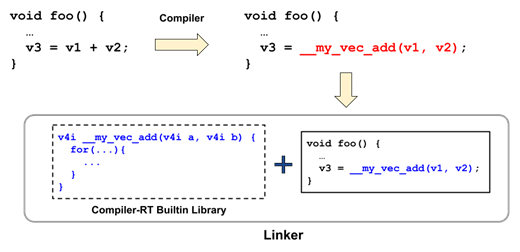
\includegraphics[width=0.6\textwidth]{content/3/chapter12/images/2.png}\\
图12.2 - 内置Compiler-RT的工作流程
\end{center}

这里显示的工作流类,似于我们在LPCSan中的需求:前一节中,我们开发了一个LLVM Pass,该Pass插入了额外的函数调用来收集循环行程计数,但是我们仍然需要实现这些收集器函数。如果使用上图所示的工作流,我们可以得出如下图所示的设计:

\hspace*{\fill} \\ %插入空行
\begin{center}
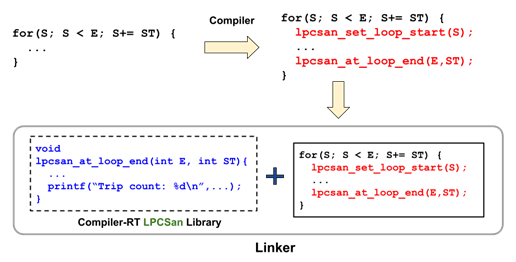
\includegraphics[width=0.6\textwidth]{content/3/chapter12/images/3.png}\\
图12.3 - Compiler-RT LPCSan组件的工作流程
\end{center}

上图显示了\texttt{\_\_lpcsan\_set\_loop\_start}和\texttt{\_\_lpcsan\_at\_loop\_end}的函数体放在一个Compiler-RT库中,这个库最终将与最终的二进制文件相链接。在这两个函数中,我们使用输入参数计算迭代计数,并输出结果。本节的其余部分中,我们将展示如何为LPCSan创建这样的Compiler-RT库。让我们开始:

\begin{itemize}
\item 首先,将文件夹切换到\texttt{llvm-project/compiler-rt},即Compiler-RT的根目录。这个子项目中,我们创建一个名为\texttt{lib/lpcsan}的新文件夹,然后再将一个新的\texttt{lpcsan.cpp}文件放入其中。在这个文件中,创建检测函数的框架:

\begin{lstlisting}[style=styleCXX]
#include "sanitizer_common/sanitizer_common.h"
#include "sanitizer_common/sanitizer_internal_defs.h"
using namespace __sanitizer;

extern "C" SANITIZER_INTERFACE_ATTRIBUTE
void __lpcsan_set_loop_start(s32 start){
	// TODO
}
extern "C" SANITIZER_INTERFACE_ATTRIBUTE
void __lpcsan_at_loop_end(s32 end, s32 step){
	// TODO
}
\end{lstlisting}

这里有两件事值得注意:首先,使用Compiler-RT提供的原始数据类型,例如:上面的代码中,我们使用\texttt{s32}—在\texttt{\_\_sanitizer}命名空间下可用—来表示有符号的32位整数,而不是普通的整数。这背后的基本原因是,我们可能需要为不同的硬件架构或平台构建Compiler-RT库,其中一些\texttt{int}的宽度可能不是32位。

其次,虽然我们使用C++来实现检测函数,但需要将它们公开为C函数,因为C函数具有更稳定的\textbf{应用程序二进制接口(ABI)}。因此,请确保在要导出的函数中添加\texttt{extern "C"}。宏\texttt{SANITIZER\_INTERFACE\_ATTRIBUTE}也确保函数将正确地暴露在库接口上,所以也请添加这个宏。

\item 接下来,向这两个函数添加必要的代码:

\begin{lstlisting}[style=styleCXX]
static s32 CurLoopStart = 0;
extern "C" SANITIZER_INTERFACE_ATTRIBUTE
void __lpcsan_set_loop_start(s32 start){
	CurLoopStart = start;
}
extern "C" SANITIZER_INTERFACE_ATTRIBUTE
void __lpcsan_at_loop_end(s32 end, s32 step){
	s32 trip_count = (end - CurLoopStart) / step;
	s32 abs_trip_count
	  = trip_count >= 0? trip_count : -trip_count;
	Report("INFO: Found a loop with "
	       "trip count %d\n", abs_trip_count);
}
\end{lstlisting}

我们在这里使用的实现非常简单:\texttt{CurLoopStart}是一个全局变量,存储当前循环的初始索引变量值,并且可以用\texttt{\_\_lpcsan\_set\_loop\_start}进行更新。

当一个循环完成时,将调用\texttt{\_\_lpcsan\_at\_loop\_end}。当发生这种情况时,在打印结果之前,我们使用存储在\texttt{CurLoopStart}中的值,以及\texttt{end}和\texttt{step}参数来计算当前循环的准确迭代计数。

\item 既然我们已经实现了核心逻辑,现在就可以构建这个库了。在\texttt{lib/lpcsan}文件夹中,创建\texttt{CMakeLists.txt}文件,并插入以下代码:

\begin{lstlisting}[style=styleCMake]
…
set(LPCSAN_RTL_SOURCES
	lpcsan.cpp)
add_compiler_rt_component(lpcsan)

foreach(arch ${LPCSAN_SUPPORTED_ARCH})
	set(LPCSAN_CFLAGS ${LPCSAN_COMMON_CFLAGS})
	add_compiler_rt_runtime(clang_rt.lpcsan
		STATIC
		ARCHS ${arch}
		SOURCES ${LPCSAN_RTL_SOURCES}
				$<TARGET_OBJECTS:RTSanitizerCommon.${arch}>
				$<TARGET_OBJECTS:RTSanitizerCommonLibc.${arch}>
		ADDITIONAL_HEADERS ${LPCSAN_RTL_HEADERS}
		CFLAGS ${LPCSAN_CFLAGS}
		PARENT_TARGET lpcsan)
	…
endforeach()
\end{lstlisting}

上面的代码中,只显示了\texttt{CMakeLists.txt}中最重要的部分。以下是一些重点:


\begin{enumerate}[label=\roman*.]
\item Compiler-RT有自己的CMake宏/函数集。在这里,我们使用它们中的两个,\texttt{add\_compiler\_rt\_component}和\texttt{add\_compiler\_rt\_runtime},分别为整个\texttt{LPCSan}创建一个伪构建目标和库构建目标。

\item 与传统的构建目标不同,如果杀毒器想在Compiler-RT中使用支持/实用程序库(例如,前面代码中的\texttt{RTSanitizerCommon}),通常链接它们的对象文件,而不是它们的库文件。更具体地说,我们可以使用\texttt{\$<TARGET\_OBJECTS:…>}指令导入支持/实用程序组件作为输入源。

\item 杀毒库可以支持多个体系结构和平台。在Compiler-RT中,我们列举了所有受支持的体系结构,并为每个体系结构创建了一个“杀毒库”。

同样,上面的代码片段只是构建脚本的一小部分。请参考我们的示例代码文件夹中完整的CMakeLists.txt文件。
\end{enumerate}

\item 为了成功构建LPCSan,我们仍然需要在Compiler-RT中做一些更改。相同文件夹中的\texttt{Base-CompilerRT.diff}补丁提供了构建杀毒器所需的所有更改。将其应用于Compiler-RT的源代码树。以下是这个补丁的摘要:

\begin{enumerate}[label=\roman*.]
\item 改变\texttt{compiler-rt/cmake/config-ix.cmake}基本上指定了LPCSan所支持的体系结构和操作系统。我们在前面的代码片段中看到的CMake变量\texttt{LPCSAN\_SUPPORTED\_ARCH}就来自这里。

\item 整个\texttt{compiler-rt/test/lpcsan}文件夹实际上是一个占位符。与LLVM不同,出于某种原因,Compiler-RT中的每个杀毒器都需要测试。因此,我们在这里放置一个空的测试文件夹,以通过这个强加的要求。
\end{enumerate}

\end{itemize}

这些是为我们的LPCSan生成Compiler-RT组件的所有步骤。

要构建我们的LPCSan库,使用以下命令:

\begin{tcblisting}{commandshell={}}
$ ninja lpcsan
\end{tcblisting}

不幸的是,在我们修改了Clang中的编译流水之前,我们无法测试LPCSan库。本节的最后一部分中,我们将了解如何实现这个任务。

\hspace*{\fill} \\ %插入空行
\noindent
\textbf{将LPCSan加入Clang}

前一节中,了解了Compiler-RT库如何为目标程序提供补充功能,或使用特殊工具(例如刚创建的杀毒器)提供帮助。这一节中,我们将把所有的东西放在一起,这样我们就可以使用LPCSan了,只需将\texttt{-fsanitize=loop-counter}标志传递给\texttt{clang}即可。

回想一下在图12.3中,Compiler-RT库需要与我们正在编译的程序相链接。另外,为了将检测代码插入到目标程序中,我们必须运行\texttt{LoopCounterSanitizer}循环。本节中,我们将修改Clang中的编译流水,以便它在特定时间运行我们的LLVM Pass,并为我们的Compiler-RT库设置正确的配置。更具体地说,下图显示了每个组件运行LPCSan需要完成的任务:

\hspace*{\fill} \\ %插入空行
\begin{center}
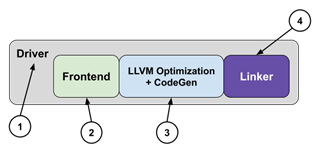
\includegraphics[width=0.7\textwidth]{content/3/chapter12/images/4.png}\\
图12.4 - 流水中每个组件的任务
\end{center}

以下是上图中每个数字的描述:

\begin{enumerate}
\item 驱动需要识别\texttt{-fsanitize=loop-counter}标志。
\item 当前端要从\textbf{抽象语法树(AST)}生成LLVM IR时,需要正确配置LLVM Pass流水,以便它包括\texttt{LoopCounterSanitizer} Pass。
\item LLVM Pass流水需要运行我们的\texttt{LoopCounterSanitizer}(如果前一个任务正确完成,不需要担心这个任务)。
\item 链接器需要将Compiler-RT库链接到目标程序。
\end{enumerate}

尽管这个工作流看起来有点复杂,但不要被这些工作所吓倒——只要提供足够的信息,Clang实际上可以完成大部分任务。在本节的其余部分中,我们将展示如何实现前面图中所示的任务,以将我们的LPCSan完全集成到Clang编译流水中(以下教程在\texttt{llvm-project/Clang}文件夹中工作)。让我们开始吧!

\begin{enumerate}
\item 首先,必须修改\texttt{include/clang/Basic/Sanitizers.def}来添加杀毒器:

\begin{lstlisting}[style=styleCXX]
…
// Shadow Call Stack
SANITIZER("shadow-call-stack", ShadowCallStack)

// Loop Counter Sanitizer
SANITIZER("loop-counter", LoopCounter)
…
\end{lstlisting}

这将有效地为\texttt{SanitizerKind}类添加一个新的枚举值\texttt{LoopCounter}。

结果是,驱动将解析\texttt{-fsanitize}命令行选项,并根据我们在\texttt{sanitizer.def}中提供的信息,自动将循环计数器转换为\texttt{SanitizerKind::LoopCounter}。

\item 接下来,让我们处理驱动部分。打开\texttt{include/clang/Driver/SanitizerArgs.h},并向\texttt{Sanit izerArgs}类添加一个新的工具方法\texttt{needsLpcsanRt}。代码如下:

\begin{lstlisting}[style=styleCXX]
bool needsLsanRt() const {…}
bool needsLpcsanRt() const {
	return Sanitizers.has(SanitizerKind::LoopCounter);
}
\end{lstlisting}

我们在这里创建的工具方法可以在驱动中的其他地方使用,以检查我们的杀毒器是否需要Compiler-RT组件。

\item 现在,让我们切换到\texttt{lib/Driver/ToolChains/CommonArgs.cpp}文件。这里,我们向\texttt{collec tSanitizerRuntimes}函数添加了几行代码:

\begin{lstlisting}[style=styleCXX]
…
if (SanArgs.needsLsanRt() && SanArgs.linkRuntimes())
	StaticRuntimes.push_back("lsan");
if (SanArgs.needsLpcsanRt() && SanArgs.linkRuntimes())
	StaticRuntimes.push_back("lpcsan");
…
\end{lstlisting}

上面的代码有效地使链接器将正确的Compiler-RT库链接到目标二进制文件。

\item 我们将对驱动做的最后一个更改是在\texttt{lib/Driver /ToolChains/Linux.cpp}中。这里,我们在\texttt{Linux::getSupportedSanitizers}方法中添加以下代码:

\begin{lstlisting}[style=styleCXX]
SanitizerMask Res = ToolChain::getSupportedSanitizers();
…
Res |= SanitizerKind::LoopCounter;
…
\end{lstlisting}

前面的代码本质上是告诉驱动,在当前的工具链(Linux的工具链)中支持LPCSan。注意,为了简化示例,我们只支持Linux中的LPCSan。如果想在其他平台和体系结构中支持这个自定义杀毒器,请修改其他工具链实现。如果需要,请参阅第8章了解更多细节。


\item 最后,我们将把\texttt{LoopCounterSanitizer} Pass插入到LLVM Pass流水中。打开\texttt{lib/CodeGe n/BackendUtil.cpp},并添加以下代码到\texttt{addSanitizers}函数中:

\begin{lstlisting}[style=styleCXX]
…
// `PB` has the type of `PassBuilder`
PB.registerOptimizerLastEPCallback(
[&](ModulePassManager &MPM,
PassBuilder::OptimizationLevel Level) {
	…
	if (LangOpts.Sanitize.has(SanitizerKind::LoopCounter))
	{
		auto FA
		=
		createFunctionToLoopPassAdaptor(LoopCounterSanitizer());
		MPM.addPass(
		createModuleToFunctionPassAdaptor(std::move(FA)));
	}
});
…
\end{lstlisting}

该文件的外围文件夹\texttt{CodeGen}是Clang和LLVM库的集合点。因此,在这里能看到几个LLVM API。这个\texttt{CodeGen}组件主要有两个任务:

\begin{enumerate}[label=\alph*.]
\item 将Clang AST转换为等效的LLVM IR模块
\item 构建一个LLVM Pass流水来优化IR和生成的机器码
\end{enumerate}

上面的代码试图定制第二个任务——即定制LLVM Pass流水。我们在这里修改的特定功能\texttt{addSanitizers},其负责将杀毒器Pass到Pass流水中。为了更好地理解这段代码,让我们关注它两个组件:

\begin{enumerate}[label=\roman*.]
\item \texttt{PassBuilder}:这个类为每个优化级别提供了预定义的Pass流水配置——即我们熟悉的O0 ~ O3符号(以及用于体积优化的Os和Oz)。除了这些预定义的布局之外,开发人员还可以利用\textbf{扩展点(EP)}自由地定制流水。

EP是(预定义的)Pass流水中的一个特定位置,可以在这里插入新的Pass。目前,\texttt{Pass Builder}支持几种EP,例如:Pass的开始、Pass的结束或向量化过程的结束等。在前面的代码中可以找到使用EP的例子,其中我们使用了\texttt{PassBuilder::registeroptimizer lastcallback}方法和一个lambda函数来定制位于Pass管道末端的EP。lambda函数有两个参数:\texttt{Mo dulePassManager}(表示Pass流水)和当前优化级别。开发者可以使用\texttt{ModulePassManager::addPass}来插入任意的LLVM Pass到这个EP中。

\item \texttt{ModulePassManager}:这个类表示一个Pass流水——或者更具体地说,是\texttt{Module}的流水。当然,对于不同的IR单元,还有其他的\texttt{PassManager}类,比如:\texttt{Function}的\texttt{FunctionPassManager}。

前面的代码中,只要\texttt{sanitierkind::LoopCounter}是由用户指定的杀毒器,就尝试使用\texttt{ModulePassManager}实例来插入我们的\texttt{LoopCounterSanitizer} Pass。因为\texttt{LoopCo unterSanitizer}是一个循环Pass,而不是一个模块Pass,所以我们需要在传递和Pa ssManager之间添加一些适配器。我们在这里使用的\texttt{createFunctionToLoopPassAda ptor}和\texttt{createModuleToFunctionPassAdaptor}函数创建了一个特殊的实例,该实例可以对不同的IR单元的PassManager进行适配。

这是Clang编译流水中支持LPCSan的所有程序逻辑。
\end{enumerate}

\item 最后,我们必须对构建系统做一些小修改。打开\texttt{runtime/CMakeLists.txt}文件,修改以下CMake变量:

\begin{lstlisting}[style=styleCMake]
…
set(COMPILER_RT_RUNTIMES fuzzer asan builtins … lpcsan)
foreach(runtime ${COMPILER_RT_RUNTIMES})
…
\end{lstlisting}

我们对\texttt{COMPILER\_RT\_RUNTIMES}所做的更改,可以将我们的LPCSan的Compiler-RT库导入到构建中。


\end{enumerate}

这些都是在Clang中支持LPCSan所必需的步骤。现在,我们终于可以使用LPCSan了:

\begin{tcblisting}{commandshell={}}
$ clang -O1 -fsanitize=loop-counter input.c -o input
\end{tcblisting}

本节中,我们了解了如何创建杀毒器。杀毒器是一种有用的工具,可以在不修改原始程序代码的情况下捕获运行时行为。创建杀毒器的能力增加了编译器开发人员,为自己的用例定制定制诊断工具的灵活性。开发杀毒器需要全面了解Clang、LLVM和Compiler-RT:创建一个新的LLVM Pass,创建一个新的Compiler-RT组件,并在Clang中定制编译流水。读者们可以使用本节的内容,来强化您在本书前几章中所学到的知识。

在本章的最后一节中,我们将再看一种工具:PGO。















